\section{Regulator}

We will be using a LM317 for the current and voltage regulations, 
as this is a cheap regulator and it is well known. 
This design will also have a 5V supply, 
which can be created from a LM7805 or with a LM317 with two resistors.

\subsection{Current Regulator}
In the datasheet of the LM317, there is a referece on how use it in a current limiting capacity as seen on figure \ref{fig:lm317_current_limit}.
\begin{figure}[ht]
    \centering
    \caption{LM317 Current-Limiter Circuit}\label{fig:lm317_current_limit}
    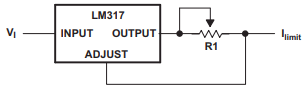
\includegraphics{img/current_limit.png}
\end{figure}

Here the current output will be 
\begin{align}
    \text{I}_{limit} &= \frac{\text{V}_{\text{ref}}}{R_{1}} \label{eq:i_limit_lm317}
\end{align}

The V$_{\text{ref}}$ is between 1.2 V and 1.3 V, and typically it is 1.25 V which is what we are going to use for calculations.
If we rearrance formula \ref{eq:i_limit_lm317} so we get $R_{1}$.
\begin{align}
    \text{I}_{limit} \cdot R_{1} &= R_{1} \cdot \frac{\text{V}_{\text{ref}}}{R_{1}} \nonumber \\
    \Downarrow  \nonumber \\
    \text{I}_{limit} \cdot R_{1} &= \text{V}_{\text{ref}} \nonumber \\
    \Downarrow  \nonumber \\
    \frac{ \text{I}_{limit} \cdot R_{1} }{\text{I}_{limit}} &= \frac{\text{V}_{\text{ref}}}{\text{I}_{limit}} \nonumber \\
    \Downarrow  \nonumber \\
    R_{1} &= \frac{\text{V}_{\text{ref}}}{\text{I}_{limit}}\\
\end{align}
So now we can calculate for the maximum current
\begin{align}
    R_{1}   &= \frac{\text{V}_{\text{ref}}}{\text{I}_{limit}} \nonumber \\
            &= \frac{1.25 \text{V}}{1.5\text{A}} \nonumber \\
            &= \underline{ \underline{ 0.8333 \Omega}}
\end{align}
As the closes resistor we can get is 0.82 $\Omega$ this is the one we are going to choose.
The next we want to calculate is the paralle resistor, this is the one which can be adjusted.